%
% This is a borrowed LaTeX template file for lecture notes for CS267,
% Applications of Parallel Computing, UCBerkeley EECS Department.
% Now being used for CMU's 10725 Fall 2012 Optimization course
% taught by Geoff Gordon and Ryan Tibshirani.  When preparing 
% LaTeX notes for this class, please use this template.
%
% To familiarize yourself with this template, the body contains
% some examples of its use.  Look them over.  Then you can
% run LaTeX on this file.  After you have LaTeXed this file then
% you can look over the result either by printing it out with
% dvips or using xdvi. "pdflatex template.tex" should also work.
%

\documentclass[twoside]{article}
\setlength{\oddsidemargin}{0.25 in}
\setlength{\evensidemargin}{-0.25 in}
\setlength{\topmargin}{-0.6 in}
\setlength{\textwidth}{6.5 in}
\setlength{\textheight}{8.5 in}
\setlength{\headsep}{0.75 in}
\setlength{\parindent}{0 in}
\setlength{\parskip}{0.1 in}

\usepackage{url}
\usepackage{graphicx}
\graphicspath{ {images/} }

%
% ADD PACKAGES here:
%

\usepackage{amsmath,amsfonts,graphicx}

%
% The following commands set up the lecnum (lecture number)
% counter and make various numbering schemes work relative
% to the lecture number.
%
\newcounter{lecnum}
\renewcommand{\thepage}{\thelecnum-\arabic{page}}
\renewcommand{\thesection}{\thelecnum.\arabic{section}}
\renewcommand{\theequation}{\thelecnum.\arabic{equation}}
\renewcommand{\thefigure}{\thelecnum.\arabic{figure}}
\renewcommand{\thetable}{\thelecnum.\arabic{table}}

\DeclareMathOperator*{\argmin}{arg\,min}

%
% The following macro is used to generate the header.
%
\newcommand{\lecture}[4]{
   \pagestyle{myheadings}
   \thispagestyle{plain}
   \newpage
   \setcounter{lecnum}{#1}
   \setcounter{page}{1}
   \noindent
   \begin{center}
   \framebox{
      \vbox{\vspace{2mm}
    \hbox to 6.28in { {\bf Notes
	\hfill } }
       \vspace{4mm}
       \hbox to 6.28in { {\Large \hfill #2  \hfill} }
       \vspace{2mm}
       \hbox to 6.28in { {\it #3 \hfill #4} }
      \vspace{2mm}}
   }
   \end{center}
   \markboth{Notes #1: #2}{ #1: #2}
}
%
% Convention for citations is authors' initials followed by the year.
% For example, to cite a paper by Leighton and Maggs you would type
% \cite{LM89}, and to cite a paper by Strassen you would type \cite{S69}.
% (To avoid bibliography problems, for now we redefine the \cite command.)
% Also commands that create a suitable format for the reference list.
\renewcommand{\cite}[1]{[#1]}
\def\beginrefs{\begin{list}%
        {[\arabic{equation}]}{\usecounter{equation}
         \setlength{\leftmargin}{2.0truecm}\setlength{\labelsep}{0.4truecm}%
         \setlength{\labelwidth}{1.6truecm}}}
\def\endrefs{\end{list}}
\def\bibentry#1{\item[\hbox{[#1]}]}

%Use this command for a figure; it puts a figure in wherever you want it.
%usage: \fig{NUMBER}{SPACE-IN-INCHES}{CAPTION}
\newcommand{\fig}[3]{
			\vspace{#2}
			\begin{center}
			Figure \thelecnum.#1:~#3
			\end{center}
	}
% Use these for theorems, lemmas, proofs, etc.
\newtheorem{theorem}{Theorem}[lecnum]
\newtheorem{lemma}[theorem]{Lemma}
\newtheorem{proposition}[theorem]{Proposition}
\newtheorem{claim}[theorem]{Claim}
\newtheorem{corollary}[theorem]{Corollary}
\newtheorem{definition}[theorem]{Definition}
\newenvironment{proof}{{\bf Proof:}}{\hfill\rule{2mm}{2mm}}

% **** IF YOU WANT TO DEFINE ADDITIONAL MACROS FOR YOURSELF, PUT THEM HERE:

\newcommand\E{\mathbb{E}}

\begin{document}
%FILL IN THE RIGHT INFO.
%\lecture{**LECTURE-NUMBER**}{**DATE**}{**LECTURER**}{**SCRIBE**}
\lecture{1}{Inverse Depth Parametrization for Monocular SLAM}{}{Sally Hui}

These are a work in progress! 

\section{Introduction}
\subsection*{Delayed and Undelayed Initialization}
Delayed initialization means adding features only when their depth uncertainty is sufficiently low. This means that they cannot be used in the map for pose estimation until they are finally added. This also means that features that are far away or close to the motion epipole may not make it into the map, as they are rejected before inclusion into the map. Previous work using this approach has involved: waiting till the measurement equation appears Gaussian; and, using a 3D semi-infinite ray in the main map to represent everything except the depth of a feature and using a particle filter to refine the estimate, but \textbf{is not added to the state vector until included} (I think this is a good point, that you can add points to the map but not include them in the state).

Undelayed initialization means new features can immediately be used to refine the motion estimate; while highly uncertain depth provides little information on translational movement, they are still very good as bearing references for rotational movement.

\subsection*{Points at Infinity}
Points at infinity exhibit no parallax due to extreme depth. Similar to above, they cannot be used to estimate camera translation, but are perfect for estimating rotation, as they are great bearings. When all features are infinite (e.g. very-large-scale outdoor scenes), SLAM turns the camera into a visual compass.

We can treat features as all starting with infinite depth, and ``coming in'' when sufficient parallax is observed. An appropriate scheme must be chosen so that finite depth can be proven given sufficient motion, and uncertainty in depth can be represented for even features with infinite depth. The reason here is that, even if we observe no parallax for a feature, that gives us a lower bound on its depth.

\subsection*{Inverse Depth Representation}
There is clearly an advantage to undelayed representation. Explicit parametrization of the \textit{inverse depth} of a feature along a semiinfinite ray from the position it was first viewed allows a Gaussian distribution to cover uncertainty in depth to nearby to infinity. Thus, it can be inserted into the map right at the start.

We use a linearity index to indicate how well low and high parallax features can be represented through inverse depth parametrization.

Inverse depth representation requires six parameters, rather than the 3 of XYZ coding. The linearity index can indicate when a feature can be safely switched back to XYZ encoding. This means that features can adopt a sort of hybrid scheme, where points that are low parallax are represented with the inverse depth parametrization, while points that are high parallax are represented with XYZ encoding.

The projective nature of a camera means that the image measurement process is nearly linear in the inverse depth coordinate. The proposed inverse depth parametrization is \textit{relative to the position from which features were first observed}, which preserves this linearity and means the Gaussian distribution is uniquely well behaved.

\section{State Vector}

\subsection*{Camera Motion}

A constant angular and linear velocity model is used to model handheld camera motion. The camera state $x_v$ is composed of pose terms: $r_{WC}$ camera optical center position and $q_{WC}$ quaternion defining orientation, and linear and angular velocity $v^W$ and $\omega^C$ relative to world frame $W$ and camera frame $C$, respectively.

The linear and angular accelerations $a^W$ and $\alpha^C$ produce impulses of linear and angular velocity:
\begin{equation}
\begin{split}
V^W &= a^W\Delta t \\
\Omega^C &= \alpha^C \Delta t \\
\end{split}
\end{equation}

The state update equation for the camera is then:
\begin{equation}
{\bf f}_v =
\left(\begin{matrix}{\bf r}^{WC}_{k+1} \cr {\bf q}^{WC}_{k+1} \cr {\bf v}^{W}_{k+1} \cr {\omega}^{C}_{k+1}\end{matrix}\right) =
\left(\begin{matrix}{\bf r}^{WC}_{k}+\left({\bf v}_k^W+{\bf V}_k^W\right)\Delta t\hfill \cr {\bf q}^{WC}_{k} \times {\bf q}\left(\left({\omega}^C_k+\Omega^C\right)\Delta t\right)\hfill \cr {\bf v}^{W}_{k}+{\bf V}^W\hfill \cr {\omega}^{C}_{k}+\Omega^C\hfill\end{matrix}\right) 
\end{equation}

The first row is simply adding the current velocity to the impulse to get an updated velocity, and using the time delta to get the change in position.

The second row is an update for the quaternion representing the rotation of the camera; ${\bf q}\left(\left({\omega}^C_k+\Omega^C\right)\Delta t\right)$ is the quaternion representing the rotation from $\left({\omega}^C_k+\Omega^C\right)\Delta t$

The two bottom rows are simply adding the current velocity to the calculated impulse.

\subsection*{Euclidean XYZ Point Parametrization}
As standard, the $i^{th}$ point is 
\begin{equation}
{\bf x}_i = \left(\!\begin{matrix}X_i & Y_i & Z_i\end{matrix}\!\right) ^ T.
\end{equation}

\subsection*{Inverse Depth Point Parametrization}

\begin{figure}[h]
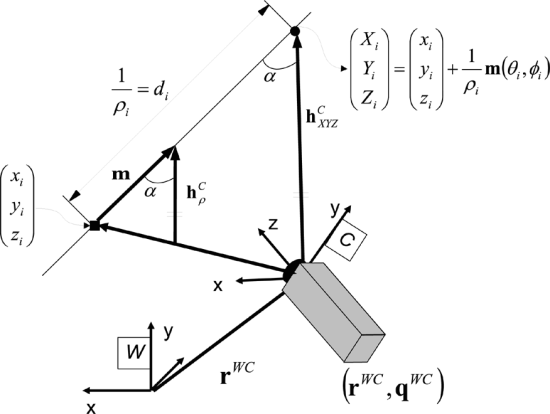
\includegraphics[scale=0.3]{inverse-parametrization.png}
\centering
\caption{Illustration of parameters, using the inverse depth scheme}
\end{figure}

A 3D point is defined by the 6-D state vector:
\begin{equation}
{\bf y}_i = \left(\!\begin{matrix}x_i & y_i & z_i & \theta_i & \phi_i & \rho_i\end{matrix}\!\right)^T.
\end{equation}

This models a 3D point located at 
\begin{equation}
{\bf x}_i = \left(\begin{matrix}X_i \cr Y_i \cr Z_i\end{matrix}\right) = 
\left(\begin{matrix}x_i \cr y_i \cr z_i\end{matrix}\right)+ {1 \over \rho_i}{\bf m}\left(\theta_i, \phi_i\right),
\end{equation}
where
\begin{equation}
{\bf m} = \left(\cos\,\phi_i \sin\,\theta_i,-\sin\,\phi_i, \cos\,\phi_i \cos\,\theta_i\right)^T.
\end{equation}

$x_i$, $y_i$, and $z_i$ are the camera optical center from which the point was first observed, and $\theta_i$ and $\phi_i$ are azimuth and elevation respectively (coded in the world frame), which defines the unit vector $m(\theta_i, \phi_i)$.

The depth along the ray $d_i$ is encoded by its inverse $\rho_i = 1/d_i$.
\begin{figure}[h]
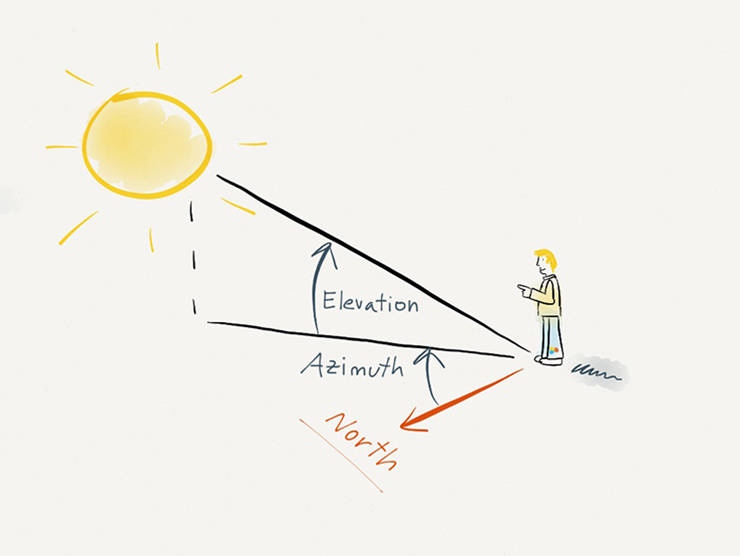
\includegraphics[scale=0.3]{azimuth.jpg}
\centering
\caption{Illustration of elevation and azimuth}
\end{figure}

\subsection*{Full State Vector}
The whole state vector contains the camera and all of the map features,
\begin{equation}
{\bf x}=\left({\bf x}_v^\top, {\bf y}_1^\top, {\bf y}_2^\top, \ldots, {\bf y}_n^\top\right)^\top . 
\end{equation}

\section{Measurement Equation}
A point $y_i(x_i)$ defines a ray coded by a direction vector in the camera frame $\textbf{h}^C = (h_x, h_y, h_z) ^ \top$.

To represent a point in XYZ coordinates in the camera frame, simply apply the transform that takes points from the world frame to camera frame. This can also be stated as subtracting the position of the camera and applying the inverse rotation that defines the pose of the camera:

\begin{equation}
{\bf h}^C={\bf h}^C_{{XYZ}}={\bf R}^{CW}\left(\begin{matrix}X_i \cr Y_i \cr Z_i\end{matrix}-{\bf r}^{WC}\right) .
\end{equation}

To represent a point inverse depth,
\begin{equation}
{\bf h}^C={\bf h}^C_{\rho}={\bf R}^{CW}\left(\rho_i\left(\left(\begin{matrix}x_i \cr y_i \cr z_i\end{matrix}\right)-{\bf r}^{WC}\right)+ {\bf m}\left(\theta_i,\phi_i\right)\right) 
\end{equation}

Compare it with Equation 1.5, which has been normalized with the inverse depth. It is normalized so that we don't divide by $\rho_i$ ($\rho_i = 0$ is safe).

The camera observes the projection of each point using the pinhole model, which gives image coordinates of
\begin{equation}
{\bf h}=\left(\begin{matrix}u \cr v\end{matrix}\right)= \left(\begin{matrix}u_0-\displaystyle{f \over d_x}{h_x \over h_z} \cr v_0-\displaystyle{f \over d_y}{h_y \over h_z}\end{matrix}\right)
\end{equation}
Where $f$ is focal length, and $d_x$ and $d_y$ are the pixel size. This is the same as our normal pinhole projection model, our $f_x = f/d_x$ and $f_y = f/d_y$.

At low parallax (that is, it is far away, $d_i$ is large and $\rho_i$ is small), Equation 1.9 reduces to 
\begin{equation}
{\bf h}^C\approx {\bf R}^{CW}\left({\bf m}\left(\theta_i,\phi_i\right)\right) 
\end{equation}

\section{Measurement Equation Linearity}

The more linear a measurement equation is, the better a Kalman filter based on it performs.

\subsection*{Linearized Propagation of a Gaussian}
We want to measure how linear a measurement equation is when evaluated around a value of a Gaussian variable. This is analagous to measuring the curvature of a multivariate function; indeed, the final expression mirrors the common expression for the curvature of a function parameterized by time. The difference is that we need to account for the Gaussian distribution of the variable, effectively by normalizing with the standard deviation.

Let $x$ be an uncertain variable with a Gaussian distribution, $x \sim N (\mu_x, \sigma_x^2)$. Transforming $x$ by $f$,

\begin{equation}
y\sim N\left(\mu_y,\sigma_y^2\right), \; \mu_y=f\left(\mu_x\right),\;\sigma_y^2=\left.{\partial f\over \partial x}\right\vert _{\mu_x} \sigma_x^2 \left.{\partial f\over \partial x}\right\vert _{\mu_x}^\top 
\end{equation}

The taylor expansion for the first derivative gives
\begin{equation}
{\partial f \over \partial x}\left(\mu_x+\Delta x\right)\approx \left.{\partial f \over \partial x}\right\vert _{\mu_x}+ \left.{\partial^2 f \over \partial x^2}\right\vert _{\mu_x}\Delta x .
\end{equation}

Comparing the value of the derivative at the interval center $\mu_x$ with the value at the extremes $\mu_x \pm 2\sigma_x$ using the linearity index,
\begin{equation}
L=\left\vert {\left.\displaystyle{\partial^2 f\over \partial x^2}\right\vert _{\mu_x}2\sigma_x\over \left.\displaystyle{\partial f\over \partial x}\right\vert _{\mu_x}}\right\vert .
\end{equation}

Although this is called a ``\textit{linearity index}'', \textbf{$L \approx 0$ indicates that the function is linear in the interval, and Gaussianity is preserved during the transformation.}

\subsection*{Linearity of XYZ Parametrization}

A point's location error $d$ is encoded as Gaussian in depth,
\begin{equation}
D = d_0+d, \qquad d \sim N\left(0,\sigma_d^2\right).
\end{equation}
\begin{figure}[h]
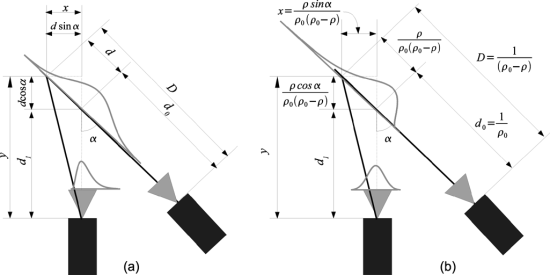
\includegraphics[scale=0.5]{uncertainty.png}
\centering
\caption{Depth uncertainty illustration}
\end{figure}

Accounting for this error $d$, the first coordinate of the 2D image of the point in the second camera is
\begin{equation}
u = {x \over y}={d\sin\,\alpha \over d_1 + d\cos\,\alpha} 
\end{equation}

Applying the same linearity index expression from 1.14 gives
\begin{equation}
L_d = \left\vert {{(\partial^2 u/ \partial d^2)}2\sigma_d\over {\partial u/ \partial d}}\right\vert ={4\sigma_d\over d_1}\left\vert {\rm cos}\,\alpha\right\vert 
\end{equation}

\subsection*{Linearity of Inverse Depth Parametrization}
Similarly, but with the depth error as Gaussian in inverse depth,
\begin{equation}
D = {1 \over \rho_0-\rho}, \qquad\rho \sim N\left(0,\sigma_\rho^2\right) 
\end{equation}

\begin{equation}
 d= D-d_0 = {\rho \over \rho_0\left(\rho_0-\rho\right)}\qquad d_0 = {1 \over \rho_0}
\end{equation}

Giving
\begin{equation}
u = {x \over y}={d\sin\,\alpha \over d_1+d\cos\,\alpha}={\rho\sin\,\alpha \over \rho_0 d_1\left(\rho_0-\rho\right)+ \rho\cos\,\alpha } 
\end{equation}

and linearity index
\begin{equation}
L_\rho = \left\vert {{(\partial^2 u/ \partial \rho^2)}2\sigma_\rho\over {\partial u / \partial \rho}}\right\vert ={4\sigma_\rho \over \rho_0}\left\vert 1- {d_0 \over d_1}{\rm cos}\,\alpha\right\vert .
\end{equation}

\section{Feature Initialization}
We assign a general Gaussian prior in inverse depth to encode that the point has to be in front of the camera.

The initial location for a newly initialized feature is
\begin{equation}
\hat{{\bf y}}\left(\hat{{\bf r}}^{WC}, \hat{{\bf q}}^{WC}, {\bf h}, \rho_0\right)=\left(\!\begin{matrix}\hat{x}_i & \hat{y}_i & \hat{z}_i & \hat{\theta}_i & \hat{\phi}_i & \hat{\rho}_i\end{matrix}\!\right)^\top 
\end{equation}
Whcih is a function of the current pose estimate $\hat{r}^{WC}$, $\hat{q}^{WC}$, and the image observation $h = (u \quad v)^\top$, which determine the depth prior$\rho_0, \sigma_0$. 

The end of the initialization ray is the current camera location estimate,
\begin{equation}
\left(\!\begin{matrix}\hat{x}_i &\hat{y}_i &\hat{z}_i\end{matrix}\!\right)^\top = \hat{{\bf r}}^{WC} 
\end{equation}

The direction of the ray is computed from the observed point in the world coordinate frame,
\begin{equation}
{\bf h}^W={\bf R}_{WC}\left(\hat{{\bf q}^{WC}}\right)\left(\!\begin{matrix}\upsilon & \nu & 1\end{matrix}\!\right)^\top
\end{equation}

Where $\upsilon$ and $\nu$ are normalized image coordinates. The angles we parametrize the direction in are 
\begin{equation}
\left(\begin{matrix}\theta_i \cr \phi_i\end{matrix}\right) = \left(\begin{matrix}\arctan\left({\bf h}_{x}^W,{\bf h}_{z}^W\right) \cr \arctan\left(-{\bf h}_{y}^W, \sqrt{{{\bf h}_{x}^W}^2+{{\bf h}_{z}^W}^2}\right) \end{matrix}\right) . 
\end{equation}

The covariances of $\hat{x}_i, \hat{y}_i, \hat{z}_i, \hat{\theta}_i$, and $\hat{\phi}_i$ are derived from the image measurement error covariance $\textbf{R}_i$ and the state covariance estimate $\hat{{\bf P}}^{{\rm new}}_{k\vert k}$.

The state covariance after feature initialization is
\begin{equation}
\hat{{\bf P}}^{{\rm new}}_{k\vert k} = {\bf J}\left(\begin{matrix}\hat{{\bf P}}_{k\vert k} & 0 & 0 \cr 0 & {\bf R}_i & 0 \cr 0 & 0 &\sigma_{\rho}^2\end{matrix}\right){\bf J}^\top
\end{equation}
\begin{equation}
 {\bf J} = \left(\left.\begin{matrix}I\cr\cr\hline\cr \displaystyle{\partial {\bf y}\over \partial{\bf r}^{WC}}, {\partial {\bf y}\over \partial{\bf q}^{WC}},0,\ldots,0,\;\;\end{matrix}\!\!\right\vert \!\!\! \begin{matrix}0 \cr\cr\hline\cr \;\;\displaystyle{\partial {\bf y} \over \partial{\bf h}}, {\partial {\bf y} \over \partial\rho}\end{matrix}\right) .
\end{equation}

\section{Switching from Inverse Depth to XYZ}

\subsection*{Conversion from Inverse Depth to XYZ Coding}
After each estimation step, the linearity index $L_d$ is computed for every map feature coded in inverse depth
\begin{equation}
{\bf h}^W_{{{{XYZ}}}} =\hat{{\bf x}}_i-\hat{{\bf r}}^{WC}\qquad \sigma_d = {\sigma_\rho \over \rho_i^2}\qquad \sigma_\rho=\sqrt{{\bf P}_{{\bf y}_i{\bf y}_i}\left(6,6\right)} 
\end{equation}
\begin{equation}
d_i = \left\Vert {\bf h}^W_{{XYZ}}\right\Vert \qquad\;\;\;\cos\alpha = {\bf m}^\top{\bf h}^W_{{XYZ}} \left\Vert {\bf h}^W_{{XYZ}}\right\Vert ^{-1}.
\end{equation}
where $\hat{\textbf{x}}_i$ and $\textbf{P}_{y_i y_i}$ is the submatrix 6x6 covariance matrix corresponding to the considered feature.

If $L_d$ is below a certain switching threshold, the feature is transformed using Equation 1.5 and the full state covariance matrix P is transformed with the corresponding Jacobian,
\begin{equation}
{\bf P}_{{\rm new}}={\bf J}{\bf P}{\bf J}^\top \qquad\;\;\;\; {\bf J}={\rm diag}\left({\bf I},{\partial {\bf x}_i \over \partial {\bf y}_i},{\bf I}\right) .
\end{equation}

\subsection*{Linearity Index Threshold}
They use $L_d < 0.1$ as a threshold to determine linearity and to switch to XYZ encoding.

\end{document}




